%\documentclass[aps,prl,preprint,superscriptaddress,showpacs]{revtex4}
\documentclass[aps,prl,reprint,longbibliography,superscriptaddress]{revtex4-1}
%\documentclass[aps,prl,reprint,longbibliography]{revtex4-1}
%\usepackage{graphicx}
 
 \usepackage{amsmath,bm}
 \usepackage{mathrsfs}
 \usepackage{amsfonts}
 %\usepackage[font=it]{caption}
 \usepackage{graphicx}
 %\usepackage{xcolor}
 \usepackage{setspace} %leaves captions single space in draft mode
 \usepackage{graphicx}
 \usepackage{epstopdf}
 \usepackage{dcolumn}
 \usepackage{amsmath}
 \usepackage{epsfig}
 \usepackage{indentfirst}
 \usepackage{psfrag}
 \usepackage{subfigure}
 %\usepackage{subcaption}
 \usepackage{amssymb}
 %\bibliographystyle{apsrev}
 \usepackage{color}
 \usepackage{units} % rz
\usepackage{soul} % strikethrough text

 \usepackage{graphicx}% Include figure files
 \usepackage{float}
 \graphicspath{{Figures/}} %Setting the graphicspath
 \usepackage{dcolumn}% Align table columns on decimal point
 \usepackage{bm}% bold math
 \usepackage{natbib}
\usepackage{multirow}

\usepackage{physics}
\usepackage{dcolumn}% Align table columns on decimal point
\usepackage{bm}% bold mathhttps://www.overleaf.com/project/5af95d0f3775594d14d4a052
%\usepackage{hyperref}% add hypertext capabilities
\usepackage{natbib}
\usepackage[backref=none,bookmarksnumbered=true,bookmarks=true,bookmarksopen=true,colorlinks=true,
citecolor=blue,linkcolor=blue,anchorcolor=green,urlcolor=blue,unicode=false]{hyperref}

%******************************* For corrections ===================
\usepackage{ulem}[normalem] %Whatch out, places underlining in Journal references. Use \normalem before references to deactivate this 
\def\red{\color{red}}
\def\black{\color{black}}
\def\blue{\color{blue}}
\def\BaCl{BaCl$_2$ }
\def\Ba{Ba$^{+2}$ }
\def\Na{Na$^{+}$ }


\normalem
\newcommand{\np}[1]{\textcolor{blue}{ #1}}
\newcommand{\npc}[1]{\textcolor{cyan}{(NP: #1)}}
\newcommand{\rw}[1]{\textcolor{cyan}{RW: #1}}
\newcommand{\str}[1]{\textcolor{cyan}{\st{#1}}}

\newcommand{\completar}[1]{{\color{red} #1}}
\newcommand{\rev}[1]{{\color{blue} #1}}

\makeatletter
\newcommand\colorsout[1]{\bgroup \markoverwith{\textcolor{#1}{\rule[0.5ex]{2pt}{0.4pt}}}\ULon}
\newcommand{\effacer}[1]{{\colorsout{red}{{\color{red}#1}}}}
\makeatother
%******************************* For corrections ===================


%******************************* Supporting Info ===================
\newcommand{\beginsupplement}{%
        \setcounter{table}{0}
        \renewcommand{\thetable}{S\arabic{table}}%
        \setcounter{figure}{0}
        \renewcommand{\thefigure}{S\arabic{figure}}%
     }
%******************************* Supporting Info ===================




\begin{document}
\title{Demonstration of On-surface Chelation of fluorescence chemo-sensors for neutrinoless detection}

   \author{Pablo Herrero}
   \affiliation{Centro de F\'{\i}sica de Materiales (CSIC/UPV-EHU), 20018 Donostia-San Sebasti\'an, Spain}
   \affiliation{Donostia International Physics Center DIPC, 20018 Donostia-San Sebasti\'an, Spain}
   \author{Maxim Ilyn}
   \affiliation{Centro de F\'{\i}sica de Materiales (CSIC/UPV-EHU), 20018 Donostia-San Sebasti\'an, Spain}
    \author{Martina Corso}
   \affiliation{Centro de F\'{\i}sica de Materiales (CSIC/UPV-EHU), 20018 Donostia-San Sebasti\'an, Spain}
   \affiliation{Donostia International Physics Center DIPC, 20018 Donostia-San Sebasti\'an, Spain}

    \author{Dimas's group people}
   \affiliation{Centro de F\'{\i}sica de Materiales (CSIC/UPV-EHU), 20018 Donostia-San Sebasti\'an, Spain}
   \affiliation{Donostia International Physics Center DIPC, 20018 Donostia-San Sebasti\'an, Spain}
 \author{Sospechosos habituales}
   \affiliation{Donostia International Physics Center DIPC, 20018 Donostia-San Sebasti\'an, Spain}
\affiliation{UPV-EHU}

  \author{Celia Rogero}
   \affiliation{Centro de F\'{\i}sica de Materiales (CSIC/UPV-EHU), 20018 Donostia-San Sebasti\'an, Spain}
   \affiliation{Donostia International Physics Center DIPC, 20018 Donostia-San Sebasti\'an, Spain}


\begin{abstract}

\completar{Por definir. Pero el abstract tiene que contener algo de información del tipo: } Using a combination of surface science techniques we demonstrate the in-vacuum chelation of the crown ether rings which, linked to a fluorescence scaffold, makes the Fluorescence Bicolor Indicator molecule (FBI). The molecules, immobilized on a surface, can trap different ions, \Ba or \Na ions, and  this process alters the molecular core level peaks, the structural conformation, as well as the electronic molecular structure, as revealed by the combination of XPS and STM/STS.
\end{abstract}

\date{\today}
\maketitle

\section{Introduction } 
Chemical sensors are miniaturised devices that can deliver real time and on-line information on the presence of specific compounds or ions in even complex samples \cite{cammann1996cambridge}. 
 Among them, optical chemical sensors employ optical transduction techniques to yield analyte information \cite{mcdonagh_optical_2008}. Due to the outstanding characteristics of both fluorescence and phosphorescence signals, they are widely applied to the construction of chemical sensors where susceptible fluorescence molecules are immobilized on a surface \cite{wolfbeis_materials_2005}.This kind of sensors has been used in many different applications in biology, medicine, environment,  \completar{.... Completar aplicaciones y referencias}. 
 
 Recently fluorescence chemo-sensors has been also proposed as useful tool in particle and nuclear physics, in particular, to establish that neutrinos are their own antiparticles \cite{majorana_teoria_2008}. \completar{aqui tal vez mencionar algo de la colaboración NEXT... esto para Juanjo} It has been proposed that the way to demonstrate this effect is by detecting the \Ba daughter produced in the decay of Xe atoms \cite{Nygren_2015} because only the double beta decay of the $^{136}$Xe isotope is expected to produce \Ba ions within a radiopure time projection chamber.
 Initially, the use of a common indicator, Fluo3, was proposed as chemo-sensor for the trapping of the \Ba ions,\cite{jones_single_2016},\cite{next_collaboration_demonstration_2018} and, nowadays, works have evolved to the design and synthesis of new functional molecules that could serve as sensors for the single ion sensing \cite{thapa_barium_2019},  \cite{thapa_demonstration_2021}. The concept includes the functionalization of a surface detector with the fluorescence molecular sensor, which, by interaction with the \Ba change their fluorescence response, either by enhancement or shift of the emitted light.  
 
 Within this context, we have recently synthesized the molecule shown in figure \ref{ModeloFBI}, the Fluorescent Bicolor Indicators (FBI). This molecule has been designed to have a strong selectivity for capturing \Ba. \cite{rivilla_fluorescent_2020} This molecule has a crown ether derivative group as trapping cage for the ions bonded to a custom-designed fluorophore. Interestingly, upon capture, not only the crown ether but also the phenyl group and the nitrogen contained in the fluorophore participate in the coordination bond with the \Ba  ion. This coordination induces a large molecular torsion with respect to the free FBI molecule (see figure \ref{ModeloFBI}). As a consequence, upon forming the \Ba  complex (chelation) the fluorescence emission spectrum gets considerably blue-shifted. This blue-shift has been measured in solution\cite{rivilla_fluorescent_2020}. Moreover, the molecules embedded in silica pellets retain their fluorescence properties when they are measured in air and has the capability of capturing sublimated \Ba.
 
 \begin{figure*}[ht!]
	\includegraphics[width=0.9\textwidth]{figures/fig1_fbi_model.pdf}
	\caption{\label{ModeloFBI} 
    Upper panel: Model of the FBI molecules before and after chelation, including the fluorescence colours in solution. Lower panel: schematic representation of the experiment we have carried out, where FBI molecules were sublimated, chelated and characterized inside the UHV chamber.}
\end{figure*}  

 In the way to develop a final chemo-sensor for barium detection, it is necessary to immobilize the molecules on a surface while preserving its ion sensitivity. Furthermore, the process must take place in the absence of any solvent, since the sensor will be installed in a high-pressure gas xenon chamber. In the present work we address this task and we demonstrate that the FBI molecules, sublimated in UHV conditions onto different substrates (see scheme in Figure \ref{ModeloFBI}, preserve their high capability to trap metal ions. By combining highly surface sensitive techniques, X-ray Photoemission Spectroscopy (XPS) and Scanning Tunneling Microscopy and Spectroscopy (STM/STS), we prove how different ions interact differently with the molecules. We demonstrate that only \Ba ions induce molecular structural changes, modify the electronic structure and therefore affect the fluorescence emission. Coordination with crown-ether happens entirely in vacuum, which ensures that chemical, structural and electronic changes are independent of solvents, air molecules or spurious contaminants. This is a crucial step toward the development of the Ba tagging sensor. Furthermore, it provides the bases to envision the application of this kind of crown ether-based chemosensors in a broad development of sensing, such as the detection of Ra atoms.

Crown ethers have been important and fundamental macrocyclic molecules in applications such as drug carriers \cite{uchegbu_non-ionic_1998} or photo-switching devices \cite{malval_photoswitching_2002}, \cite{uda_membrane_2005}. Because of their capability to capture a variety of guest species, including metal cations, protonated species and neutral and ionic molecules \cite{dobler1980ionophores}, crown ethers \cite{gokel_crown_1991} have been extensively used in solution, or even in gas phase to recognize and trap metal or molecular ions \cite{more_intrinsic_1999}, \cite{maleknia_cavity-size-dependent_2002}. However, despite their unique coordinating properties, crown ethers have been poorly exploited in solid state. Few examples can be found in the literature where self-assembled monolayers of crown ether derivatives have been grown and used on surfaces. Moreover, in all previous studies, either the growth or ion trapping or both has taken place in solution \cite{yoshimoto_hostguest_2003}, \cite{flink_recognition_1999}, \cite{inokuchi_new_2015}. 
 There are only two works, as far as we know, where crown ethers were deposited under ultra high vacuum conditions (UHV) \cite{feng_growth_2018} and their metal trapping capability was proven also under UHV \cite{stredansky_-surface_2019}. In the latter work, reactivity of the crowns upon anchoring on an organic template on Au(111) is carefully explored. In addition, by combining XPS and STM, they probe that the crown ethers, assembled into a regular 2D guest–host array, can successfully trap sodium atoms.

\section{Results and discussion}
%Esta separación por apartados/subapartados luego puede aparecer o no, dependiendo de a que revista lo mandemos, pero por ahora la dejo porque ayuda a escribir y ordenar las ideas. Luego se puede reestructurar para que el mensaje llegue de la mejor manera posible.

\subsection{Chemical probe of chelation}
Prior to addressing the chelation of the molecule, we start by confirming that FBI molecules are sublimated intact on the substrate. Figure \ref{XPS_FBI_Au(111)} a) shows the molecular core levels of FBI molecules, i.e. O 1s, N 1s and C 1s. The spectra were measured for 0.65 ML deposited on Au(111) at RT. The ratios between the three core levels are in agreement with having stoichiometric molecules on the surface (C/O = 6.2, C/N = 10.3). The C 1s core level, which appears centered at around 285 eV, can be fitted using two components, one centered at around 284.7 eV and a second and more intense one at 286.3 eV, with relative intensities in agreement with having intact molecule. The former component corresponds to C-C bonds whereas the component at higher binding energy (B.E.) includes contributions from C-O and C-N. In the N 1s region, around 400 eV, a faint peak is visible. The position of the maxima is compatible with the two amida groups of the molecular composition. Finally, the O 1s core level present a single component peak centered at 532.8 eV.

\begin{figure*}[ht!]
	\includegraphics[width=0.9\textwidth]{figures/fig2_xps_chelation.a).png}
	\includegraphics[width=0.4\textwidth]{figures/XPS_O1s_evolution_Au.png}
	
	%\includegraphics[width=0.5\textwidth]{XPS_O1s_evolution_Au.png}
	\caption{\label{XPS_FBI_Au(111)} 
    XPS spectra on O 1s, N 1s and C 1s regions measured after 0.65 ML FBI deposition on Au(111) (a); after their chelation with 1.46 \Ba per FBI molecule (b) and 1.43 \Na per FBI molecule (c). Evolution of chelated component as a function of the \Ba deposition (d)}
\end{figure*}  

For the chelation, \BaCl was sublimated on the FBI functionalized Au(111) surface. It is worth mentioning that upon sublimation, the stoichiometry of the salt does not remain 1:2 but rather 2:1. This means that mainly \Ba is deposited on the surface (see S.I. for details).
After sublimation of 1.46 \Ba per FBI molecule, the core levels, shown in figure \ref{XPS_FBI_Au(111)} b), are clearly shifted toward higher B.E, mainly on O 1s and N 1s

The maximum O 1s core level exhibits an upward shift of 0.5 eV. This shift is not just a doping shift, but a real chemical change. This is revealed by the evolution of the O 1s for very low \Ba doses on the surface. Figure \ref{XPS_FBI_Au(111)} shows the O 1s evolution for \Ba ions amounts below 1 \Ba per FBI molecule. The peak width increases as \Ba is added to the sample: the peak of the free molecule (prior to \Ba addition) has a FWHM of 2.04, whereas it has a FWHM of 2.20 for the lattest state, with 0.63 \Ba per FBI. Thus, we deconvolve the peaks after \Ba addition using two components, one at 533.2 eV (FWHM = 2.20) corresponding to the free molecules and another at 533.8-534.0 eV, corresponding to chelated molecules.   This is consistent with the molecules undergoing a chemical change upon chelation, rather than a surface doping shift due to adding the ions. \completar{The relative contribution of the component from the chelated molecules may be expected to depend on the amount of barium deposited. However, the resolution of the current experiments limited our assessment of this dependency.}. The contribution to the O 1s peak from the neighbouring Au 4p was subtracted using the spectrum of the clean Au. More information can be found in the supplementary information.

In the only reference paper were crown ether deposited on Au(111) were chelated, ref. \cite{stredansky_-surface_2019} Stredansky and coworkers observed higher shifts in the O1s core level, which gradually shifts up to around 1 eV by increasing the amount of deposited atoms (\Na in their case). 
To evaluate whether the nature of the dopant atom has any influence in the oxygen core level shift for the FBI molecules, we tested the chelation with Na. Thus, figure \ref{XPS_FBI_Au(111)} c) shows the O 1s, N 1s and C 1s core levels measured on 0.6 ML of FBI on Au(111) before and after the sublimation of 1.43 \Na per FBI. The maximum O 1s shift for \Na-chelated FBI molecules is again 0.5 eV, excluding the nature of the ion as responsible of the shift.
It is noteworthy to remember here that in REF \cite{stredansky_-surface_2019} crown ether groups were oriented parallel to the Au substrate without any possibility to move or rotate. By contrast, in our case, as we will discuss later, the crown ethers have more flexibility and mobility and can adopt any conformation with respect to the surface. In fact, this mobility and flexibility are also reflected in the N 1s core level, which exhibits a shift in the case of \Ba-chelation but not in the case of \Na-chelation.
According to theoretical calculations, upon chelation with \Ba, the FBI undergo a structural torsion promoting that the iminic N atom at the fluorophore interact with the ions \cite{rivilla_fluorescent_2020}.  For the case of \Na the ion does not produce the torsion given its smaller size. The \Na ion does not  occupy all coordination spots, it does not interact either with the iminic N atom or the phenyl ring. \completar{Fernando: he redactado esta parte (Pablo), ¿lo he entendido bien? \textbf{FER: OK, ya he lanzado el cálculo con Na(+)}}



\subsection{Molecular aspect and electronic changes induced by chelation}

\completar{This part is tobe written by Dimas's group. We } The XPS results represent the first evidence of ion trapping by FBI molecules in total absence of any solvent. Second and unambiguous probe is the visualization of the structural and electronic changes that FBI molecules undergone upon chelation. And the best tool to see these changes is the STM. Figure \ref{STM_FBI_fluorophore} a) shows the aspect of the Au(111) after the sublimation of XXXX ML FBI. Molecules tend to aggregate forming islands and individual molecules are difficult to identify. The islands crosses the steps, which are not special absorption position for the molecules. An example of this individual molecules is shown in the the HR-STM image (CO tip, constant height, XXXXX mV) Figure \ref{STM_FBI_fluorophore} b). In this image the fluorofore is clearly distinguished, while the crown ether is very difficult to be measured because crown ether is freely moving. 
Since this molecule is not flat, it is difficult to obtain a good HR-STM image. To compare and to identify the different parts of the molecule, the fluorophore and fluorophore with phenyl ring were also sublimated. In the image we see ..... \completar{Discuss about the STM image of the FBI as well as images for the fluorophore and fluorophore with phenyl ring.}

\begin{figure*}[ht!]
	\includegraphics[width=0.9\textwidth]{figures/STM_FBI_fluoroforos.png}
	\caption{\label{STM_FBI_fluorophore} 
    Idea for the STM image. Here Dimas/Patrick change the figure as you consider. }
\end{figure*}  

Figure \ref{STM_chelation} shows the STM image of FBI before and after \Ba deposition... together with the STS... \completar{Discuss about the molecular changes after chelation as well as relate the electronic changes with the changes in the fluorescence and relate this changes with the structural changes.}

\begin{figure*}[ht!]
	\includegraphics[width=0.9\textwidth]{figures/fig4_stm_chelation.png}
	\caption{\label{STM_chelation} 
    Idea for the STM image. Here Dimas/Patrick change the figure as you consider. }
\end{figure*}  

\completar{If we include the calculation, then include a discussion about them.\textbf{ FER: OK, we can include the HOMO-LUMO gaps and the theoretical emission spectra for FBI and FBI·Ba(2+) to connect the structural changes (geometry) with the computational photophysics.}}



\subsection{FBI chelation independent of the surfaces}

Finally we have also tested that chelation is taken place also in other surfaces, in particular Cu(111) and ITO. We chose Cu(111) because it is a more reactive substrate. This enabled us to study whether the molecule-substrate interaction could alter the chelation response. On the other hand, ITO was selected because it is a transparent substrate which allows the direct detection of fluorescence. \completar{Furthermore, the conductivity of ITO could enable guiding the \Ba ions towards the surface in order for the molecules to capture it. These properties make ITO a promising candidate for the potential implementation of the Ba-tagging sensor on a Time Projection Chamber (TPC) \cite{rivilla_fluorescent_2020}}.

As we saw before, the O 1s shift can be used as fingerprint of the chelation. Figure \ref{XPS_FBI_Cu_ITO} shows the O 1s core level measured for FBI deposited on Cu(111) and ITO. For Cu(111) we observed the same chemical shift on the O 1s (0.7 towards higher BE), indicating that chelation was also happening. In this case, the core level has a small component at lower B.E., around 531 eV, which is associated to residual contamination of the Cu surface in the form of Cu$_2$O \cite{zhu_surface_2013}.
The analysis of the shift for the case of ITO was not as direct because of the presence of oxygen in the ITO structure. To assess the differences associated to the FBI and chelated FBI molecules the core level measured on the ITO as prepared  was subtracted from that measured with FBI and BaCl$_2$. The result of the subtraction is shown in figure \ref{XPS_FBI_Cu_ITO} b), and the inset gathers the original normalized spectra, including the contribution from the ITO. From the 0.9 eV shift towards higher B.E. in figure \ref{XPS_FBI_Cu_ITO} b), we see that chelation is also taking place in ITO. These results ensure that chelation is independent from the choice of substrate, and that it is a property intrinsic to the molecule in conjugation with \Ba. 
\completar{Terminar con una frase muy general para remarcar la importancia de hacerlo en distintas superficies}  


\begin{figure*}[ht!]
	\includegraphics[width=0.95\textwidth]{figures/fig5_cu_ito.png}
	\caption{\label{XPS_FBI_Cu_ITO} 
    a) O 1s core level spectra measured for FBI on Cu(111) and ITO surfaces before and after \Ba sublimation. For ITO the substrate O 1s core level were substrates to emphasize the O 1s contribution coming from FBI.}
\end{figure*}  


\section{Experimental Procedure}

 The molecular evaporations were done on three Au(111), Cu(111) and Indium Tin Oxide (ITO). The surfaces were cleaned by cycles of sputtering and annealing and their cleanness was checked by XPS prior to FBI deposition. FBI, \BaCl and NaCl were evaporated from homemade knudsen cells. To avoid cross talking between FBI and the salts molecules and to exclude any possibility of chelation of the molecule inside the cell, the FBI and \BaCl  evaporators were located in two separated parts of the chamber.
 
The evaporation thickness was estimated by studying the attenuation of the most intense substrate core level, i.e. Au 4f, Cu 2p and In 3d. The calculations followed the guidelines provided in ref. \cite{powell_practical_2020}. For this purpose, we estimated the Electron Effective Attenuation (EAL) of electrons through the FBI layers for electrons with kinetic energies of 1402.6, 1041.6 and 554.61 eV (Au 4f 5/2, In 3d 5/2 and Cu 2p 3/2). The resulting EALs are 3.87, 3.05 and 1.85 nm, respectively. The thickness of the FBI samples was then estimated using the intensity of clean substrate core level as reference and the attenuated intensity after the evaporation. The amount of \Ba (Na) per molecule were estimated by computing  the ratio $\theta=I_{Ba}/3I_N \cdot S_N/S_Ba $, where $I_{Ba}$, $I_N$ is total area  of the  Ba 3d  and  N 1s  core  levels and $S_Ba = 7.49$, $S_N = 0.47$ are the corresponding atomic sensitivity factors\cite{Moulder1992HandbookOX}. The factor 3 corresponds to considering 3 N atoms per molecule.

The XPS measurements were carried out using a SPECS Phoibos 100 electron analyzer, using a non monochromatic Al K$\alpha$ photon source, (1486.6 eV).Three different substrates were use: Au(111), Cu(111) and  ITO/quartz. The three were cleaned in UHV by sputtering annealing cycles and the cleanness were tested by XPS before deposition of FBI. The spectra were calibrated to the substrates main core level (Au 4f, Cu 2p, and In 3d, respectively). 

\bibliographystyle{apsrev4-1} 
\bibliography{literature_FBI}


\section{Supplementary Information}
\subsection{Data processing for O 1s on Au(111)}
\begin{figure*}[ht!]
	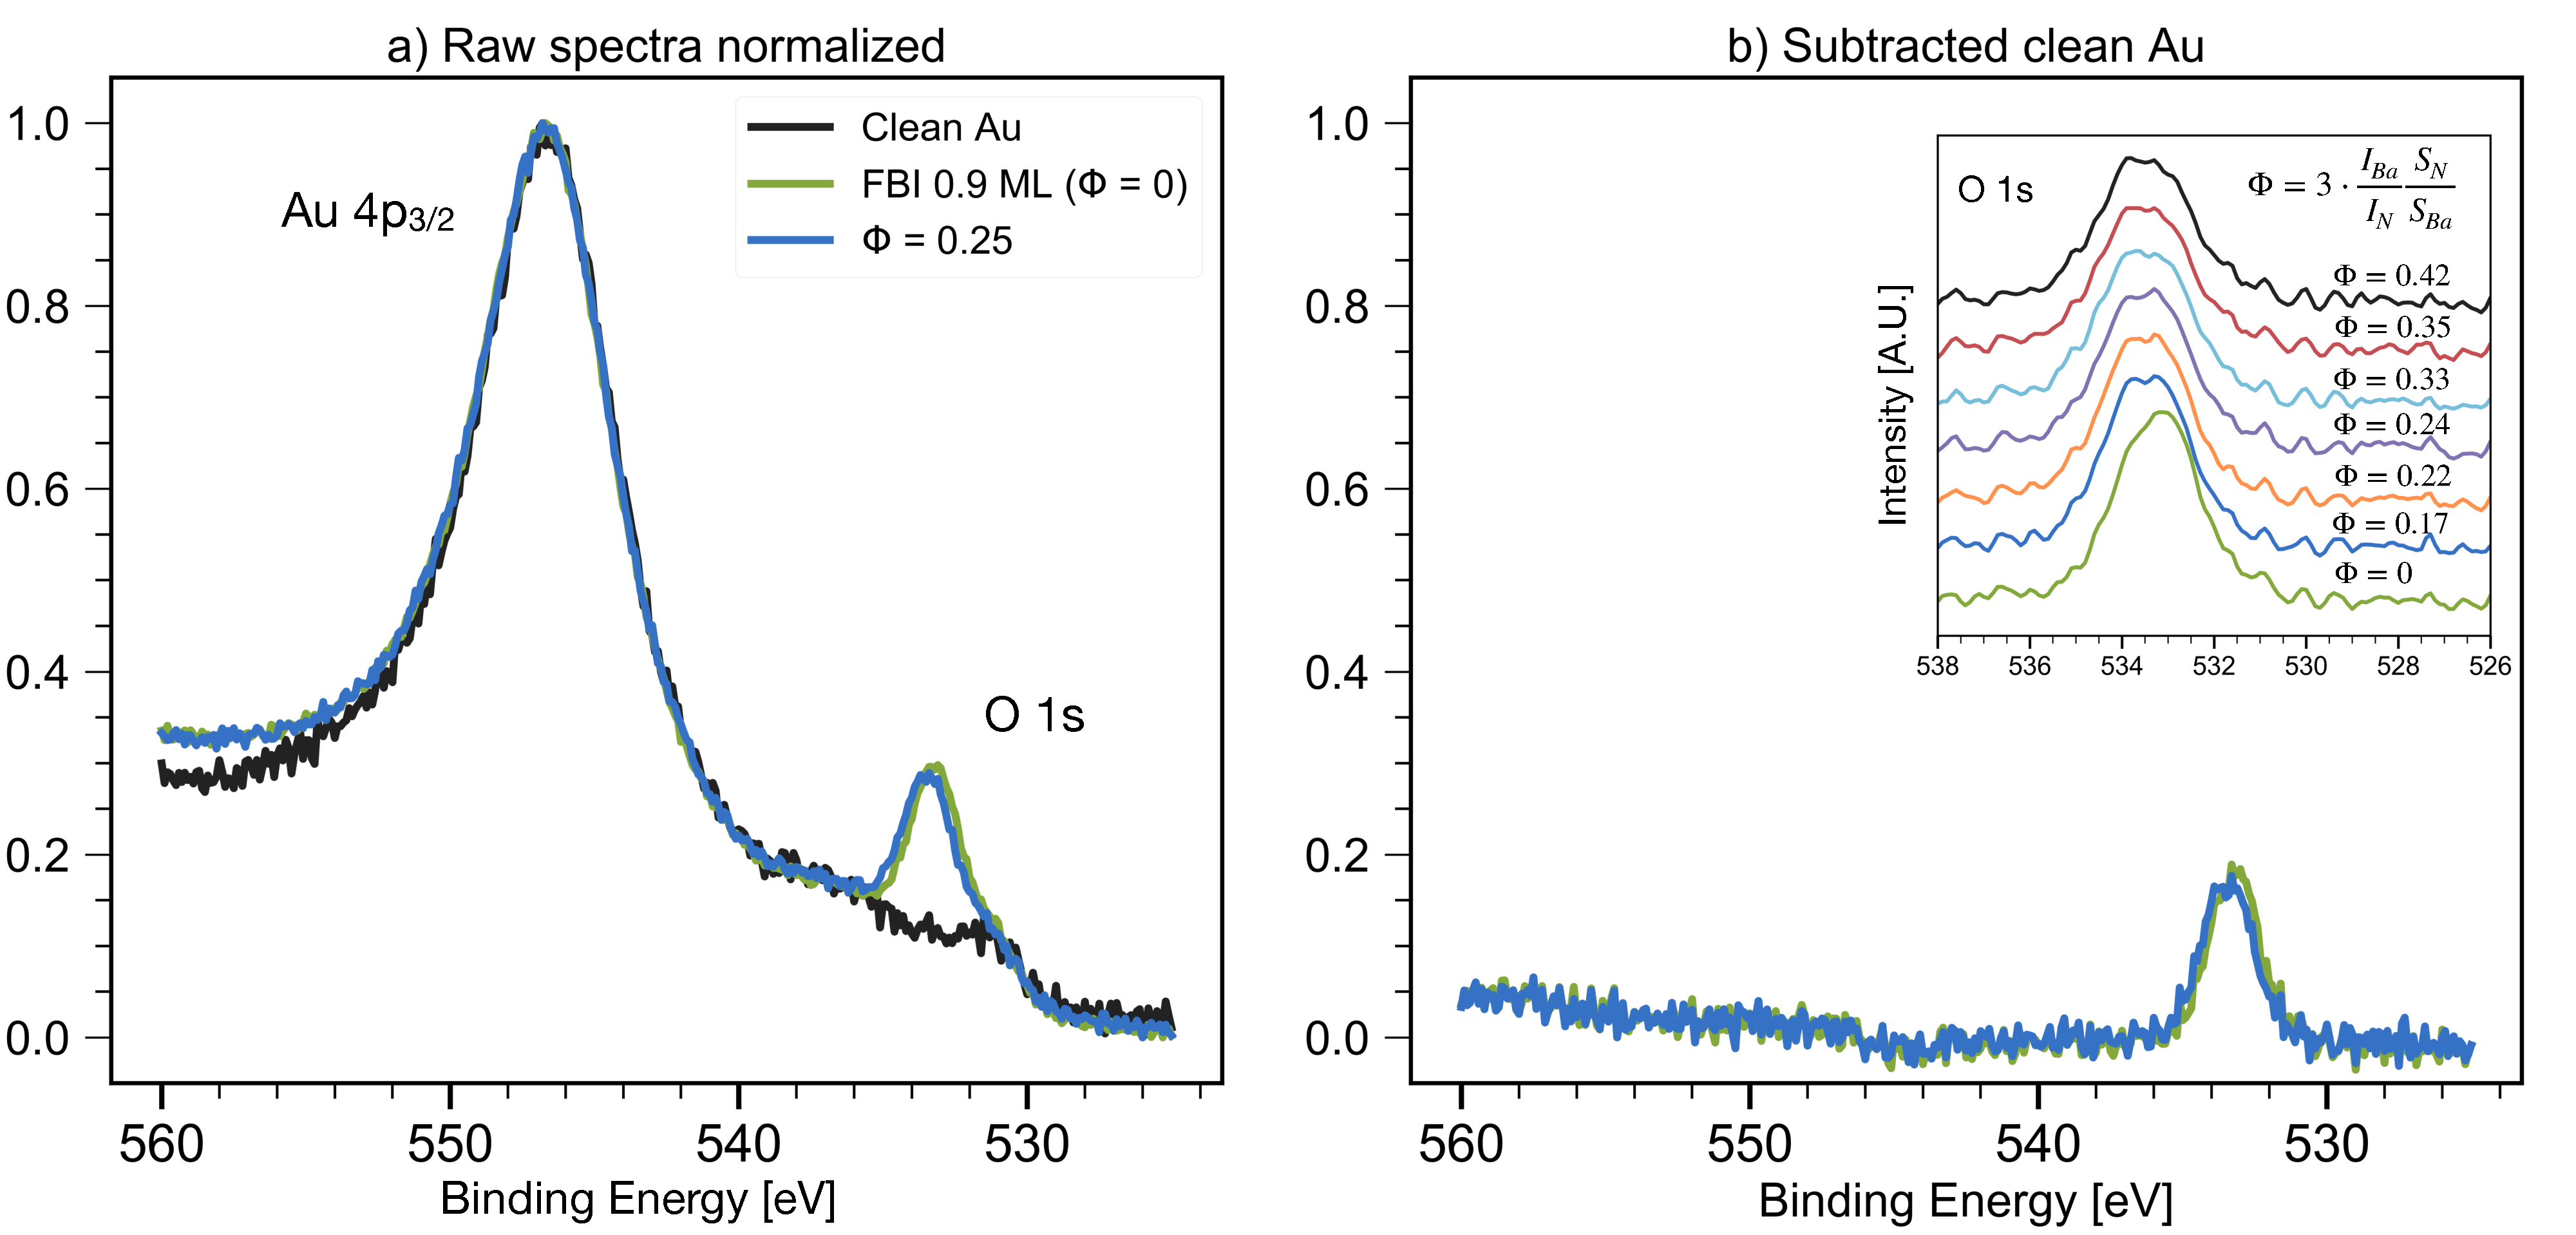
\includegraphics[width=0.9\textwidth]{figures/si_au_subtraction.png}
	\caption{\label{Au_subtraction} 
    XPS data treatment for O 1s core level in Au(111). The Au 4p core level contributes to the O 1s background. The intensity of the clean sample (red line) was subtracted from that corresponding to the deposition of FBI molecule (green line). To account for the attenuation of the Au 4p peak after evaporating the molecule, the maximum intensity of both curves was normalized to unity. The same treatment was applied to all lines in figure \ref{XPS_FBI_Au(111)} d). Those curves are shown here as inset with no offset.}
\end{figure*}  

\subsection{Calculation of the Ba:Cl stoichiometry after sublimation}

\begin{figure*}[ht!]
	\includegraphics[width=0.9\textwidth]{figures/si_bacl_au_cu.png}
	\caption{\label{Chlorine_desorption} 
    Evaporation of \BaCl directly (with no FBI molecule layer in between) on Cu(111) (black line) and Au(111) (red line). The stoichiometry ratio Cl/Ba, taking into account the atomic sensitivity factors (0.89 and 7.49 for Cl 2p and Ba 3d, respectively) is 0.7 and 0.64, for deposition in Au and Cu, respectively. Compare this to the expected ratio of 2 for the stoichiometric \BaCl salt.}
\end{figure*}  

\end{document}
